\documentclass[12pt]{article}
\usepackage{ebgaramond}
\usepackage{graphicx}
\usepackage{microtype}

\title{Cupid and Psyche\footnote{Excerpted from books \textsc{iv} through
\textsc{vi} of \textit{The Metamorphosis, or The Golden Ass.}}}
\author{Apuleius \and Thomas Taylor (tr.)\footnote{T.~Taylor. \textit{The
Metamorphosis, or Golden Ass, and Philosophical Works of Apuleius.} R.~Triphook
and T.~Rodd, 1822.}}
\date{}

\begin{document}
\maketitle

\noindent In a certain city lived a king and a queen, who had three daughters
of conspicuous beauty.\footnote{This fable, which was designed to represent the
lapse of the soul from the intelligble world to the earth, was certainly not
invented by Apuleius: for, as it will appear in the course of this note, it is
\textit{evidently} alluded to by Synesius, in his book on Dreams, and
\textit{obscurely} by Plato and Plotinus. It is clear, therefore, that Plato
could not derive his allusion from Apuleius; and as to Plotinus and Synesius,
those who are at all acquainted with the writings of the Greek philosophers,
well know that they never borrowed from Latin authors, from a just conviction
that they had the sources of perfection among themselves.

I have said, that this fable represented the lapse of the human soul; of the
truth of which, the philosophical reader will be convinced by the following
observations. In the first place, the Gods, as I have elsewhere shown, are
super-essential natures, from their profound union with the first cause, who is
super-essential without any addition. But though the Gods, through their
summits or unities, transcend essence, yet their unities are participated
either by intellect alone, or by intellect and soul, or by intellect, soul, and
body; from which participations the various orders of the Gods are deduced.
When, therefore, intellect, soul, and body, are in conjunction, suspended from
this super-essential unity, which is the centre, flower, or blossom, of a
divine nature, then the God from whom they are suspended is called a mundane
God. In the next place, the common parents of the human soul are the intellect
and soul of the world; but its proximate parents are the intellect and soul of
the particular star about which it was originally distributed, and from which
it first descends. In the third place, those powers of every mundane God, which
are participated by the body suspended from his nature, are called mundane; but
those which are participated by his intellect, are called super-mundane; and
the soul, while subsisting in union with these super-mundane powers, is said to
be in the intelligible world; but when she wholly direct her attention to the
mundane powers of her God, she is said to descend from the intelligible world,
even while subsisting in the heavens.

Thus much being premised, let us proceed to the explanation of the fable.
Psyche, then, or soul, is described as transcendantly beautiful, and this is
indeed true of every human soul, before it profoundly merges itself in the
defiling folds of dark matter. In the next place, when Psyche is represented as
descending from the summit of a lofty mountain, into a beautiful valley, this
signifies the descent of the soul from the intelligible world into a mundane
condition of being, but yet without abandoning its establishment in the
heavens. Hence, the palace which Psyche beholds in the valley, is, with great
propriety, said to be ``a royal house, which was not raised by human, but by
divine hands and art.'' The gems too, on which Psyche is said to have trod in
every part of this palace, are evidently symbolical of the stars. Of this
mundane, yet celestial condition of being, the incorporeal voices which
attended upon Psyche, are likewise symbolical: for outward discourse is the
last image of intellectual energy, according to which the soul alone operates
in the intelligible world. As voices, therefore, they signify an establishment
subordinate to that which is intelligible, but so far as denudated of body,
they also signify a condition of being superior to a terrene allotment.

Psyche, in this delightful situation, is married to an invisible being, whom
she alone recognises by her ears and hands. This invisible husband proves
afterward to be Cupid or Love; that is to say, the soul, while established in
the heavens, is united to love of the purest kind, \textit{i.~e.}~to
intellectual love, or, in other words, is not fascinated with outward form. But
in this beautiful palace she is attacked by the machinations of her two
sisters, who endeavour to persuade her to explore the form of her unknown
husband. The sisters, therefore, signify those two powers of the irrational
part of the soul, \textit{anger} and \textit{desire}, the latter of which
powers is well defined by the Pythagoreans to be a certain tendency, impulse,
and appetite of the soul, in order to be filled with something, or to enjoy
something present, or to be disposed according to some sensitive energy; just
as \textit{reason} or the rational soul is signified by Psyche. The stratagems
of these sisters at length take effect, and Psyche beholds and falls in love
with Love; that is to say, the rational part, through the incentives of anger
and desire, becomes enamoured of, and captivated with, outward form; in
consequence of which Cupid, or intellectual love, flies away, and Psyche, or
the rational soul, is precipitated to earth. It is remarkable that Psyche,
after falling to the ground, is represented as having \textit{``a stumbling and
often reeling gait;''} for Plato in the Ph{\ae}do says, that the soul is drawn
into body with a \textit{staggering} motion.

After this, commence the wanderings of Psyche in search of Cupid, or
intellectual love, from whose embraces she is unhappily torn away. In the
course of her journey, she arrives at the temples of Ceres and Juno, whose aid
she suppliantly implores. Her conduct, indeed, in this respect, is highly
becoming. For Ceres comprehends in her essence Juno, who is the fountain of
souls; and the safety of the soul arises from converting herself to the divine
sources of her being.

In the next place, Venus is represented desiring Mercury to proclaim Psyche
through all lands, as one of her female slaves, that had fled from her service.
It is likewise said that she gave him a small volume, in which the name of
Psyche was written, and every other particular respecting her. Now, I think, it
cannot be doubted that Synesius alludes to this part of the fable, in the
following passage from his treatise on Dreams: ``When the soul descends
spontaneously to its former life, with mercenary views, it receives servitude
as the reward of its mercenary labours. But this is the intention of descent,
that the soul may accomplish a certain servitude to the nature of the universe,
prescribed by the laws of Adrastia, or inevitable fate. Hence, when the soul is
fascinated with material endowments, she is affected in a manner similar to
those who, though born free, are, for a certain time, hired to employments,
and, in this condition, captivated with the beauty of some female servant,
determine to act in a menial capacity, under the master of their beloved
object. Thus, in a similar manner, when we are profoundly delighted with
external and corporeal good, we confess that the nature of matter is beautiful,
who marks our assent in her secret book; \textit{and if, considering ourselves
as free, we at any time determine to depart, she proclaims us deserters,
endeavours to bring us back, and, openly presenting her mystic volume to the
view, apprehends us, as fugitives from our mistress}. Then, indeed, the soul
particularly requires fortitude and divine assistance, as it is no trifling
contest to abrogate the confession and compact which she has made. Besides, in
this case, force will be employed; for the material inflicters of punishments
will then be roused to revenge, by the decrees of fate, against the rebels to
her laws.''

Venus, however, must not be considered here as the nature of matter; for though
she is not the celestial Venus, but the offspring of Dione, yet, according to
Proclus in Cratylum, she is that divine power which governs all the
co-ordinations in the celestial world and the earth, binds them to each other,
and perfects their generative progressions, through a kindred conjunction. As
the celestial Venus, therefore, separates the pure soul from generation, or the
regions of sense, so she that proceeds from Dione binds the impure soul, as her
legitimate slave, to a corporeal life.

After this, follows an account of the difficult tasks which Psyche is obliged
to execute, by the commands of Venus; all which are images of the mighty toils
and anxious cares which the soul must necessarily endure after her lapse, in
order to atone for her guilt, and recover her ancient residence in the
intelligible world. In accomplishing the last of these labours, she is
represented as forced to descend even to the dark regions of Hades; which
indicates that the soul, through being enslaved to a corporeal life, becomes
situated in obscurity, and is deprived of the light of day, \textit{i.~e.}~of
the splendour of truth and reality; agreeably to which Empodocles sings,

\begin{verse}
``I fled from deity and heavenly light,\\
To serve mad discord in the realms of night.''
\end{verse}

\noindent But Psyche, in returning from Hades, is oppressed with a profound
sleep, through indiscreetly opening the box given her by Proserpine, in which
she expected to find a portion of divine beauty, but met with nothing but an
infernal Stygian sleep. This obscurely signifies, that the soul, by expecting
to find that which is truly beautiful in a corporeal and terrene life, passes
into a profoundly dormant state; and it appears to me, that both Plato and
Plotinus allude to this part of the fable, in the following passages, the
originals of which may be seen in p.~10 of my Dissertation on the Eleusinian
and Bacchic Mysteries. In the first place, then, Plato, in book vii.~of his
Republic, observes, ``that he who is not able, by the exercise of his reason,
to define the idea of \textit{the good}, separating it from all others, and
piercing, as in a battle, through every kind of argument; eagerly striving to
confute, not according to opinion, but according to essence, and, in all these,
marching forward with undeviating reason,---such a one knows nothing of
\textit{the good itself}, nor of any good whatever; but if he has attained to
any image of \textit{the good}, we must say he has attained to it by opinion,
not by science; that in the present life he is sleeping, and conversant with
dreams, and that, before he is roused, \textit{he will descend to Hades, and
there be profoundly and perfectly laid asleep}.'' And Plotinus, in
Ennead.~I.~lib.~viii.~p.~80, says, ``The death of the soul is for it, while
merged, as it were, in the present body, to descend into matter, and be filled
with its impurity, and, after departing from this body, to lie absorbed in its
filth, till it returns to a superior condition, and elevates its eye from the
overwhelming mire. \textit{For to be plunged into matter, is to descend to
Hades, and fall asleep}.''

Cupid, however, of \textit{intellectual love}, at length recovering his
pristine vigour, rouses Psyche, or \textit{the rational part of the soul}, from
her deadly lethargy. In consequence of this, having accomplished her destined
toils, she ascends to her native heaven, becomes lawfully united to Cupid (for,
while descending, her union with him might be called illegitimate), lives the
life of the immortals, and the natural result of this union is pleasure or
delight. And thus much for an explanation of the fable of Cupid and Psyche. For
farther particulars respecting the lapse of the soul, see my introduction to,
and translation of, Plotinus on the Descent of the Soul, and my Dissertation on
the Eleusinian and Bacchic Mysteries.} Of these, the two elder, though of the
most agreeable form, were not thought too lovely to be celebrated by the
praises of mankind; but the beauty of the younger sister was so great and
illustrious, that it could neither be expressed, nor sufficiently praised by
the poverty of human speech. At length, a multitude of the citizens, and
abundance of strangers, whom the rumour of the exalted spectacle had collected
together, full of ardent zeal, stupid with admiration of her inaccessible
beauty, and moving their right hand to their mouths, while their forefinger was
placed on their erect thumb, venerated her with religious adorations, as if she
had been the Goddess Venus herself.

And now fame had pervaded the neighbouring cities and contiguous regions, and
had reported that the Goddess whom the azure profundity of the deep brought
forth, and the dew of the foamy billows nourished, now, every where exhibiting
her divinity, was conversant with the midst of the people; or certainly, that
once more, from a new blossom of the celestial stars, not the sea, but the
earth, had produced another Venus, endued with virginlike flower. Thus opinion
increased immensely every day; thus extended fame wandered over the
neighbouring islands, a great part of the continent, and a multitude of
provinces. Now many mortals, by long journeys on the land, and over the deep
passages of the sea, came to behold the glorious specimen of the age; no one
sailed to Paphos, no one to Cnidus, nor even to Cythera, for the spectacle of
the Goddess Venus. The sacred concerns of the Goddess were abandoned, her
temples were deformed, her ceremonies neglected, her images uncrowned, and her
desolate altars defiled with frigid ashes, while a girl was supplicated in her
stead, and the divinity of so great a Goddess was appeased in a human
countenance; and the name of the absent Venus was propitiated in the morning
progressions, victims, and banquets of the virgin. And now the people
frequently assembling in the streets, and throwing flowers entwined in
garlands, or loosely scattering them, prayed to her divinity.

% FIXME: I may want to transcribe Book XI as well, should I note the reference?
This immoderate translation of celestial honours to the worship of a mortal
virgin, inflamed the vehement mind of the true Venus; so that, impatient of
indignation, and raging high with her agitated head, she thus discoursed with
herself: ``Behold the ancient parent\footnote{See the Notes on Book XI.} of the
nature of things, lo, the first origin of the elements; behold the bountiful
Venus of the whole universe, the honour of whose majesty is divided with a
mortal girl, and whose name, raised to the heavens, is profaned by sordid
terrestrials. Indeed, by sharing in common the expiations which are offered to
divinity, I sustain an uncertain part of deputed veneration, and a girl
obnoxious to mortality bears about my celestial image. It is in vain that the
shepherd [Paris], whose justice and faith the mighty Jupiter approved,
preferred me to such great Goddesses,\footnote{The well known fable to which
this alludes, is thus beautifully unfolded by the Platonic Sallust, in his
golden treatise on the Gods and the World. ``In this fable, which is of the
mixed kind, it is said, that Discord at a banquet of the Gods threw a golden
apple, and that a dispute about it arising among the Goddesses, they were sent
by Jupiter to take the judgement of Paris, who, charmed by the beauty of Venus,
gave her the apple in preference to the rest. But the banquet denotes the
super-mundane powers of the Gods; and on this account they subsist in
conjunction with each other. And the golden apply denotes the world, which, on
account of its composition from contrary natures, is not improperly said to be
thrown by Discord, or strife. Again, however, since different gifts are
imparted to the world by different Gods, they appear to contest with each other
for the apple. And a soul living according to sense (for this is Paris), not
perceiving other powers in the universe, says, that the beauty of Venus alone
is the contended apple.''} on account of my illustrious form. But she who thus
rejoices, whosoever she be, shall not usurp my honours; for I will cause her to
repent of her illicit beauty.'' And immediately she calls her son; that winged
and sufficiently rash youth, who, with his depraved manners condemning public
discipline, armed with flames and arrows, running through other men's houses by
night, and corrupting the matrimony of all, commits such mighty wickedness with
impunity, and effects nothing useful and good.

Him, though haughty by genuine license, she stimulates by her words: she brings
him to the city, and openly shows him Psyche, (for this was the name of the
girl,) and having him the whole tale concerning the emulation of her beauty,
groaning and raging with indignation, ``I beseech thee,'' says she, ``by the
leagues of maternal love, by the sweet wounds of thy arrow, by the mellifluous
burnings of that flame, to afford thy parent full revenge, through your
reverence of me, and severely punish that rebellious beauty. Above all,
willingly effect this one thing, that the virgin may be detained by the most
ardent love of the lowest of mankind, whom fortune has deprived of his dignity,
patrimony, and safety; and so infirm that he may not find his equal in misery
throughout the world.'' Having thus spoke, and for a long time, and closely
embraced her son with ardent kisses, she sought the neighbouring margin of the
refluent shore, and, with rosy feet, trod on the topmost dew of the vibrating
waves.

Behold, now the water of the profound sea was appeased from its vertex, and the
marine train which she just began to wish, appeared without delay, as if she
had previously commanded its attendance. The daughers of Nereus were present,
singing chorus; and Protunus,\footnote{By Portunus here, or Portumnus, who, by
the Greeks, was called Pal{\ae}mon, Neptune is denoted, as the Delphin editor
well observes. For Pal{\ae}mon, who is properly Portunus, is shortly after
mentioned as being present.} rough with his cerulean beard, and Salacia, heavy
with her fishy bosom, small Pal{\ae}mon, the charioteer of a dolphin, the
company of Tritons, every where furrowing the sea; and while this softly blows
his sounding shell, that, with a silken covering, resists the unfriendly ardour
of the sun, another carries a mirror before the eyes of his mistress, and
others swim under the two-yoked car. Such was the train which attended Venus,
proceeding to the ocean.

In the meantime, Psyche perceived no advantage to herself from her admirable
beauty; she was seen by all, and praised by all; yet no one, neither kings nor
nobles, nor any one of the common people, approached as a suitor for her
possession in marriage. They admired, indeed, her divine form, but they all
admired it as an image artificially polished. Some time prior to this, her two
sisters, whose moderate beauty had not been celebrated by mankind, having been
married to suitor kings, now obtained happy nuptials; but the virgin Psyche,
sitting desolate at home, lamented her deserted solitude, sick in her body and
wounded in her soul; and, though pleasing to all nations, she hates her beauty
in herself. But the most miserable father of the most unfortunate daughter,
suspecting the celestial hatred, and fearing the wrath of the Gods, questioned
the most ancient oracle of the Milesian God,\footnote{\textit{i.~e.}~Of Apollo,
who had a temple and oracle at Miletus, a city bordering on Ionia and Carin.}
and sought of so great a divinity, by prayers and victims, nuptials and a
husband for the sorrowful virgin. Apollo, therefore, though a Grecian and
Ionian, on account of the builder of Milesia, gave the following oracle, in
Latin verse:

\begin{verse}
Of some high mountain's craggy summit place\\
The virgin, deck'd for deadly nuptial rites;\\
Nor hope a son-in-law of mortal race,\\
But a dire mischief, viperous and fierce;\\
Who flies through {\ae}ther, and with fire and sword\\
Tires and debilitates whate'er exists,\\
Terrific to the powers that reign on high.\\
E'en mighty Jove the wing'd destroyer dreads,\\
And streams and Stygian shades abhor the pest.
\end{verse}

\noindent The king, whose days, till then, had been crowned with felicity, on
hearing this sacred oracle, returned slowly home, oppressed with sorrow, and
disclosed to his wife the mandates of unpropitious fate. Many days were passed,
on this occasion, in grief, weeping, and lamentation. But the cruel injunctions
of the dire oracle now require to be accomplished. Now preparations were made
for the deadly nuptials of the most miserable virgin; now the nuptial was
changed into a funeral torch, and the sound of the Zygian\footnote{Juno, the
guardian of the bonds of wedlock, was called \textit{Zygia}, which signifies a
yoke.} [or conjugal] pipe into the querulous Lydian measure. The joyful
hymeneal song closed with mournful howling, and the wretched bride wiped away
her tears with her own nuptial veil. The whole city likewise lamented the sad
destiny of the royal house, and public mourning was immediately proclaimed on
the occasion.

The necessity, however, of complying with the celestial mandates, importunately
urged the miserable Psyche to her destined punishment. The solemnities,
therefore, of the mournful marriage being accomplished with extreme sorrow, the
living funeral takes place, followed by all the people, and the weeping Psyche
attends not her nuptials, but her obsequies. However, while her sorrowful
parents, who were overwhelmed with such a mighty evil, endeavoured to delay the
execution of the nefarious sentence, she herself exhorted them to a compliance,
in the following words: ``Why do you torture your unhappy old age with
long-continued weeping? Why do you waste your spirits, which, indeed, are more
mine than yours, with such frequent groans? Why do you deform your
countenances, which in my sight are so venerable, with unavailing tears? Why do
you lacerate my eyes in your own? Why do you thus tear your hoary hairs? Why
thus beat your venerable breasts? These must be the rewards which you are to
receive of my surpassing beauty, the truth of which having suffered a deadly
blow from villanous envy, you, too late, perceive. Alas! then should you have
wept and lamented, then bewailed me as one lost, when the people and nations
celebrated me with divine honours, and when, with one voice, they called me a
new Venus. I now perceive, I now clearly see, that I perish through the name of
Venus alone. Lead me away, and place me on the rock to which I am destined by
the oracle; I am in haste to accomplish these happy nuptials; I am in haste to
see this my noble husband. Why do I delay? Why do I avoid his approach, who is
born for the destruction of the whole world?''

The virgin, having thus spoke, was silent, and, with undaunted steps, mingled
herself with the splendid procession of the people that followed her. They
advance to the destined rock of a lofty mountain, on the summit of which,
having left the royal maid alone, with the nuptial torches extinguished with
their tears, they returned home, with dejected heads and desponding hearts. And
her miserable parents, indeed, sinking under the weight of such a mighty
calamity, shut up the gates of their palace, hid themselves in darkness, and
abandoned themselves to a perpetual night. But the mild gales of the
gently-blowing Zephyr gradually raised Psyche, as she stood, trembling and
weeping, on the summit of the rock, her garments through the tranquil breath of
the God, orbicularly expanding, and bearing her through the hollows of a
valley, at the bottom of the mountain, softly reclined her on the bosom of a
flowery turf.

Psyche, therefore, agreeably reclining in the flowery valley, on a bed of dewy
grass, the mighty perturbation of her mind being appeased, enjoyed delightful
repose. And, being now sufficiently refreshed with sleep, she rose with a more
composed mind, and saw a grove, thick planted with vast and lofty trees, and a
fountain in the middle of the grove, gently falling with glassy water.  Near
the lapse of the fountain there was a royal house, which was not raised by
human, but by divine hands and art. You might know, from the very entrance of
the palace, that you beheld the splendid and pleasant residence of a God. For
the lofty ceilings, which were curiously arched with citron-wood and ivory,
were supported by golden pillars; and all the walls were ornamented, in every
part, with silver carving, beasts of various kinds presenting themselves to the
view, in the vestibule of the palace. Wonderful was the man, indeed, and endued
with prodigious skill; or, rather, it was some demigod or God, who fashioned
the silver carving with such exquisite subtility of art.

But the very pavement itself consisted of small shells, admirably decorated
with pictures of various kinds. Blessed, thrice blessed, are those who tread on
gems and bracelets! The other parts, too, of this wide-extended and regularly
disposed palace were precious, beyond all price; and the walls being every
where strengthened with bars of gold, were so refulgent with their own
splendour, that, even in the absence of the sun, they made for the palace a day
of its own; so bright were the bedchambers, the porches, and the folding doors.
The furniture, too, was answerable to the majesty of this abode; so that it
might very properly be considered as a celestial palace, built by mighty
Jupiter, for his correspondence with mankind.

Psyche, invited by the delightful aspect of the place, approached to it, and,
assuming a little more confidence, entered within the threshold of the place.
Presently after, being allured by the charms of the beautiful vision, every
thing she surveyed filled her with admiration: and, in the more elevated part
of the house, she beheld a magnificent repository, in which immense riches were
contained. Indeed, there is not any thing in this universe with which this
place is not replete. But amidst the admiration which such prodigious wealth
excited, this was particularly wonderful, that this treasury of the whole world
was not secured by any bars, or doors, or guards.

Here, while the eyes of Psyche were ravished with delight, a voice, denudated
of its body, thus addressed her: ``And why, my mistress,'' it said, ``are you
astonished at such vast riches? All these are yours. Betake yourself,
therefore, to your bedchamber, and refresh your wearied limbs on the bed, and,
when you think proper, repair to the bath; for we, whose voices you now hear,
are your servants, who will diligently administer to all your commands, and,
while we wait on your person, prepare royal banquets for your repast.''

Psyche perceived the goodness of divine providence, and, complying with the
admonitions of the incorporeal voices, first refreshed herself with sleep, and
afterwards with the bath. Immediately, too, perceiving, in an adjacent
semicircular building, near an elevated seat, every apparatus requisite for
supper, she willingly reclined herself, considering this place as acommodated
to her refreshment; and, instantly, nectareous wines, and numerous dishes of
various kinds of food, were served in, without any visible attendants, by the
mere impulse of a certain spirit; Psyche, at the same time, perceiving no one,
but alone hearing certain words, and having voices alone for her servants.
After the table was furnished with this splendid banquet, a certain person
entered, and sang, without being seen; at the same time an invisible musician
played on the harp; and, last of all, her ears were ravished with a full
chorus, from an invisible band.

After these pleasures were finished, the evening now persuading to repose,
Psyche retired to her bed; and when the night was far advanced, a certain
gentle sound approached her ears. Then, fearing for her virginity, on account
of the profound solitude of the place, she trembles, and is filled with horror,
and dreads that of which she is ignorant beyond any calamity. And now her
unknown husband approached, ascended the bed, made her his wife, and hastily
left her before the rising of the morning light. Immediately the attendant
voices, who were the ministers of the bedchamber, took care of every thing
necessary on the occasion. This course was continued for a long time; the
novelty, by its constant repetition (as it was natural it should), became at
last delightful; and the sound of the uncertain voices was the solace of her
solitude.

In the meantime, the parents of Psyche grew old in unwearied sorrow and
lamentation; and the report of her destiny becoming more widely extended, her
elder sisters came to know all the particulars respecting it, and immediately,
being overwhelmed with sorrow, hastened to the presence of their afflicted
parents. On that very night, the husband of Psyche thus addressed her (for the
hands and the ears were the only media of their present communication): ``Most
charming Psyche, and dear wife, more cruel fortune threatens thee with a deadly
danger, which, I think, ought to be guarded against with the utmost attention.
For now your sisters, who are disturbed through the belief of your death, in
consequence of endeavouring to discover the place of your abode, will soon
arrive at the rock on which you were lately exposed. If you should chance to
hear any of their lamentations, neither make them any reply, nor even turn your
eyes towards them; for, by doing otherwise, you will be the cause of the
greatest grief to me, and of extreme destruction to yourself.''

Psyche assented, and promised that she would act agreeably to her husband's
desire. But as soon as he, together with the night, were fled, the most
miserable Psyche consumed the whole day in tears and lamentations, exclaiming
that she was now entirely lost, since, securely confined in a blessed prison,
she was deprived of human conversation, and not permitted to give salutary
assistance to her sorrowing sisters, nor even so much as to see them. Neither
refreshing herself, therefore, with the bath, nor with food, but weeping
abundantly, she retired to rest. But her husband coming more early than usual,
and embracing her weeping, thus expostulated with her: ``Is this, my Psyche,
what you promised me? What can I, your husband, now expect from you? What can I
now hope for, since, neither by day nor by night, nor even in the midst of our
conjugal embraces, you cease to be tormented with grief? But come, act now as
you please, and comply with the pernicious desires of your soul. However, when
you begin too late to repent of your folly, call to mind my serious
admonitions.''

Psyche after this had recourse to prayers, and, while she threatens that she
shall die if her request is denied, extorts from her husband permission to see
her sisters, to assuage their grief and enjoy their conversation. Thus he
pardoned the entreaties of his new wife, and permitted her, besides, to present
her sisters with as much gold and as many jewels as she pleased; but he again
and repeatedly admonished her, with the utmost earnestness, not to be
persuaded, by their pernicious advice, to inquire concerning the form of her
husband; not by a sacrilegious curiosity hurl herself from such an exalted
fortune, and by this means deprive herself of his embraces.

She thanked her husband for his indulgence, and becoming in consequence of it
more joyful; ``But,'' says she, ``may I suffer death a hundred times rather
than be deprived of thy most pleasing embraces; for I love thee most
vehemently, thee, whoever thou art, even as I love my own soul, nor would I
compare thee to Cupid himself. But this also I beseech you, grant to my
prayers, that your servant Zephyr may convey my sorrowful sisters in the same
manner in which he brought me hither.'' Then, pressing his lips with persuasive
kisses, murmuring alluring words, and fondly folding him in her arms, she thus
addressed him, in soothing accents: ``My dear husband, sweet soul of thy
Psyche, be not averse to my request.'' The husband, vanquished by the power of
Venus, reluctantly gave his consent, and promised that all things should be
accomplished according to her desire; and afterwards, in consequence of the
approach of morning, vanished from the arms of his wife.

But the sisters, having inquired the way, arrived in haste at the lofty rock on
which Psyche was left abandoned, and there wept and beat their breasts, till
the rocks resounded with their repeated lamentations. And now they called on
their miserable sister, by her proper name, till the spreading sound of their
mournful voices, gliding down the declivities of the mountain, reached the ears
of Psyche, who, distracted and trembling, ran out of her palace, and thus
addressed them, ``Why do you in vain afflict yourself with miserable
lamentations? I, whom you deplore, am now present; cease, therefore, your
complaints, and at length dry up those tears which you have so long shed for my
loss, since you may now embrace her whom you have so vehemently mourned.''

Then, calling Zephyr, she acquaints him with her husband's commands, who,
entirely obedient to the mandate of Cupid, brought them, borne on the most
gentle gales, in safety to Psyche. Now they embrace and are embraced, and
mingle their mutual caresses with frequent and hasty kisses; and the joy of
finding her alive, after they had considered her as dead, soon put a period to
their lamentations and tears. ``But come,'' said Psyche, ``enter with me into
my house, and recreate your afflicted mind with your Psyche.'' Having thus
spoken, she led them into her golden palace, brought their ears acquainted with
the populous family of voices that were subservient to her commands, and
sumptuously refreshed them in a most beautiful bath, and with the delicacies of
her immortal table. But as soon as her sisters were satiated with this
affluence of celestial riches, they began to nourish envy profoundly in their
hearts: and, at last, one of them, with a very particular and curious
importunity, inquired who was the master of these celestial possessions? And
who, and what sort of a person her husband was?

Psyche, however, by no means violated her husband's injunctions, or suffered
them to depart from the secret recesses of her bosom; but, devising an answer
adapted to the occasion, told them that he was a beautiful youth, whose cheeks
were yet only shadowed with down, and that he was, for the most part, occupied
in rural employments, and in hunting on the mountains. And lest, by any slip in
the course of her conversation, she should betray the secret advice, having
loaded them with rich presents of gold and jewels, she called Zephyr, and
ordered him to carry them to the lofty rock. This being immediately
accomplished, these admirable sisters, as they were returning home, burning
with the rancour of increasing envy, discoursed much with each other, and at
last one of them thus began: ``Do but take notice how blind, cruel, and unjust,
fortune has proved! Were you, my sister, pleased to find that we, though born
of the same parents, should maintain such a different rank in life? We, who are
elder, are delivered over to be servants to husbands, in a foreign country, far
exiled from our native land and parents; but this youngest sister, the
offspring of exhausted vigour, is raised to the enjoyment of this prodigious
affluence, and of a God for her husband, though she does not know how to use,
in a proper manner, such an abundance of good. You saw, sister, what a
prodigious quantity of bracelets the house contained, what a number of shining
garments, what bright gems, and what heaps of gold she treads upon in every
part of the palace. If to all this she possesses a husband so beautiful as she
asserts him to be, no one in the universe can live a happier life than herself.
Indeed, it may happen, through long-continued association, and corroborated
affection, that her husband, who is a God, may at length make her a Goddess. By
Hercules, it must be so, for she already conducts herself in a lofty manner;
and the woman certainly breathes the Goddess, who has voices for her servants,
and commands even the winds themselves. But I, miserable creature, am, in the
first place, tied to a husband more aged than my father; and, in the next
place, to one who is balder than a gourd, and shorter than a pigmy, and who
secures every part of his house with bolts and chains.''

``But I,'' replied the other sister, ``am destined to endure a husband, whose
body is distorted with an articular disease; and though on this account he
seldom rewards my pains with conjugal embraces, yet I am forced to spend a
great part of my time in rubbing his distorted fingers, which are almost
hardened into stone, with f{\oe}tid fomentations, defiling these delicate hands
with nasty rags and stinky poultices; thus acting the part of a surgeon more
than that of a wife. You, indeed, my sister, seem to bear all this with a
patient or rather servile soul, (for I will speak what I think, without
restraint,) but, for my own part, I can no longer endure that such a blessed
destiny should have fallen to one who does not deserve it. For only recollect
in what a proud and arrogant manner she behaved towards us. By her boasting and
immoderate ostentation, she betrayed the haughtiness of her swelling mind; of
her immense riches gave us but a very trifling part; and immediately after,
being weary of our company, ordered us to be turned out of doors, and to be
puffed and hissed away. But I am not a woman, nor do I breathe, if I do not
hurl her headlong from such mighty possessions. And if our contumely affects
you as it ought, let us both join, in vigorous consultation, how we may
accomplish this design. In order to this, let us neither acquaint our parents,
nor any one else, with our intention, nor inform them that we know any thing of
her safety. It is sufficient that we ourselves have seen what it repents us to
have seen, and let us not be the messengers of her happy condition to our
parents and the people; for those are not properly blessed whose riches no one
is acquainted with. She shall know that we are not servants, but her elder
sisters. And now, indeed, let us depart to our husbands, and visit our poor
habitations, for such they are when compared with her abode, and being
furnished with more compressed thoughts, let us return with greater firmness to
the punishment of her pride.''

The two wicked sisters consider this evil advice as good, and concealing the
precious gifts which they had received from Psyche, dishevelling their hair,
tearing their faces with dissembled grief, and renewing fictitious tears,
returned to their parents. These, however, the wounds of whose sorrows they had
again opened by their narration, they hastily take their leave of, big with the
madness of envy, and return to their own habitations, machinating nefarious
guile, or rather parricide, against their innocent sister.

In the meantime Psyche's unknown husband thus again admonished her in his
nocturnal discourses: ``Do you perceive what a mighty danger fortune is
preparing for you at a distance, and which, unless you are more firmly guarded
against than you have hitherto been, will soon assault you near at hand? Those
perfidious she-wolves are, with mighty endeavours, forming base strategems
against you, the sum of which is, that they may persuade you to explore my
countenance, which, as I have often told you, if you once see, you will see no
more. If, therefore, those worst of sorcerers come again, armed with noxious
minds, (and I know they will come), avoid all discourse with them; but if
through genuine simplicity and tenderness of disposition, you are not able to
accomplish this, at least be careful not to hear nor answer any inquiries
concerning your husband. For now we shall have a family of our own, and thy as
yet infantine womb is pregnant with an offspring, which, if you conceal my
secrets in silence, will be divine, but if you profane them, will be mortal.''

Psyche rejoiced in the consoling thoughts of a divine offspring, and was elated
with the glory which would result from her future pledge, and with the dignity
of a maternal name. She, therefore, anxiously numbered the increasing days and
departing months, and being ignorant in every thing relative to conception,
wondered how her wealthy womb could receive such an abundant increase.

But now those pests and most cruel furies, her sisters, breathing viperous
virulence, and hastening their departure, sailed with impious celerity. Then
again the momentary husband thus admonished his Psyche; ``The last day, and the
most extreme misfortune, are now arrived. The malicious sex, and hostile blood,
have taken arms, removed their camp, drawn the army into battle array, and
sounded the charge. Now, thy nefarious sisters are aiming with a drawn sword at
thy throat. Alas! most dear Psyche, what mighty calamities now press upon us?
Take pity, both on yourself and me; and by a religious continence of tongue,
deliver your house, your husband, yourself, and our little one, from the
misfortune of impending ruin. Neither see, nor hear those wicked women, who,
after the deadly hatred which they have conceived against thee, and having
trampled on the ties of blood, deserve not to be called sisters, when, like the
Sirens, standing on the mountain, they shall make the rocks resound with their
deadly voices.''

Psyche, in words interrupted by sighs and tears, thus replied: ``You have for
some time had convincing proofs of my fidelity and taciturnity; and the
strength of my mind shall be no less approved by you in the present instance.
Only order Zephyr to repeat his former office, and at least grant me the sight
of my sisters, since I am not permitted to behold thy sacred image. By thy
fragrant and every way pendulous locks! By thy cheeks tender, smooth, and like
my own! By thy breast glowing with I know not what kind of heat! By my hopes of
at least knowing thy face in this little one, I beseech thee to comply with the
pious prayers of thy suppliant, indulge me in the desired embraces of my
sisters, and recreate with joy the soul of Psyche who is devoted to thy will;
for then I shall no longer be anxious to explore thy countenance. Now nothing
can hinder me from thy embrace, not even the darkness of night, for I hold
thee, my life, in my arms.''

The husband being fascinated by these words, and by her soft embraces, wiped
away her tears with his fragrant locks, assured her that her desires should be
fulfilled, and immediately anticipated the light of the emerging day. But the
two sisters who were confederates in mischief, without calling on their
parents, direct their course with precipitate velocity from the ships to the
rock, and not waiting for the assistance of the elevating wind, leap on high
with licentious temerity. Zephyr, however, not unmindful of the royal mandate,
though unwilling to execute it, restored them, reclining on the bosom of the
gently blowing gales, to the appointed place. Then, with feet equally rapid,
they enter the palace, concealing the foe under the name of sister, embrace
their prey, and veiling a treasury of profoundly hidden fraud under a joyful
countenance, thus flattered her: ``Psyche, not now so slender as you were
before, since you are now almost a mother, what mighty good do you think you
bear for us in your womb? With what prodigious joy will you exhilarate the
whole of our house! O how happy shall we be through the nurture of the golden
infant, who, if he corresponds in beauty as he ought to do to his parents, will
be born a perfect Cupid.''

Thus, by a dissembled affection, they gradually invade the soul of their
sister, who, as soon as they had refreshed themselves from the fatigue of their
journey with warm baths, regaled them on a couch in a most splendid manner with
all the dainties of a royal banquet. She ordered a harp to speak, and some one
immediately sang to its harmony; flutes to be blown, and they immediately
sounded; a musical band to sing in chorus, and it instantly sang; and, though
invisible, ravished the souls of the hearers with the most mellifluous notes.

But the malice of these wicked women was not softened by the honeyed sweetness
of the music; but turning their discourse to the destined fraudulent snares,
they begin in a dissembling manner to inquire what sort of a person she was
married to, and from what family he was descended. Then she, through her too
great simplicity, having forgot the former account which she had given of her
husband, invented a new story respecting him. She told them that her husband
was of the next province; that he carried on a trade with abundance of money;
and that he was now of a middle age, a grey hair being here and there scattered
on his head. And without prolonging the conversation any further, she again
committed them to the charge of the winds, after she had loaded them with
costly presents. But while they return home, sublimely riding on the tranquil
breath of Zephyr, they thus discoursed with each other: ``What can we say,
sister, of the monstrous lies of that foolish creature? At one time her husband
is a young man, with the down just beginning to spread over his chin, and at
another time he is of a middle age, shining with hoary hairs. Who can this be,
that in a short space of time experiences the alteration of a sudden old age?
You may depend on it, my sister, that this vile woman either forged this lie to
deceive us, or that she does not herself know the form of her husband. But
whichever of these is the case, she must be deprived of these riches with the
utmost expedition. Indeed, if she is really ignorant of the form of her
husband, she must have married a God, and through this pregnancy of hers, she
will present us with a God. However, should she happen to be the mother of a
divine offspring, which heaven forbid! I should immediately hang myself. Let
us, therefore, in the meantime return to our parents, and by a well-coloured
deceit, prevent them from apprehending our design.''

The sisters thus inflamed, having called on their parents in a hasty manner,
and passed through a night of interrupted sleep; fly as soon as it was morning
to the rock, and by the usual vehicle of the wind, descend rapidly down to
Psyche, who, with forced tears, they thus craftily addressed: ``Happy in your
own imagination, and blessed only in your ignorance of evil, you sit here
inattentive to your own danger. But we, who watch over your affairs with a
vigilant care, are miserably tormented at your lost condition. For, by diligent
search, we have discovered, (nor can we conceal from you the cause of our
mutual grief, and your own misfortune), that a vast serpent who glides along
the plain in various volumes, whose neck is swoln with noxious poison, and
whose mouth widely gapes through profound gluttony, secretly sleeps with you by
night. Now call to mind the Pythian oracle, which declared you was destined to
marry a fierce and terrible beast; and many of the inhabitants of this place,
who haunt all round the country, have observed him returning home from his prey
in the evening, and gliding through the shallows of the neighbouring river.
These declare, that he will not long feast you with delicious delicacies, but
that, as soon as a full womb shall have given maturity to your pregnancy, he
will then devour you as a richer morsel. So that you have only to consider
whether you will comply with the desires of your sisters, who are anxious for
your dear preservation, and avoiding death, live with us secure from danger, or
be buried in the bowels of a most cruel beast. But if you are wedded to the
vocal solitude of this country retreat, or to the filthy and dangerous
enjoyment of clandestine venery, and the embraces of a poisoned serpent, we
have at least acted like pious sisters in thus admonishing you of your
danger.''

Then the miserable Psyche, as being full of simplicity, and of a pliant
disposition, is seized with terror at the dire relation, and being thus quite
beside herself, loses the remembrance of all her husband's admonitions and her
own promises, and hurls herself headlong into a profound abyss of calamity.
Trembling, therefore, and pale, and with an almost lifeless voice, she thus
addressed them in broken words: ``You, indeed, most dear sisters, have acted as
it was proper you should, with becoming piety towards me; and it appears to me
that those who gave you this information, did not invent a lie. For I have
never yet beheld my husband's face, nor do I know who or what he is; but only
hearing him by night, I endure a husband of an uncertain condition, and one
that perpetually avoids the light of day. I am, therefore, of your opinion,
that he is some monstrous beast, who always terrifies me from attempting to
behold him, and threatens some prodigious evil as the consequence of curiosity
respecting his countenance. Now, therefore, if you are able to give any
salutary assistance to your sister, who is thus dangerously situated, defer it
not for a moment.''

These wicked women, having thus found an avenue to their pernicious design, by
a full discovery of their sister's condition, laying aside the concealments of
covered artifice, invade the trembling thoughts of the simple girl with the
drawn sword of deception. At length, therefore, one of them thus began: ``Since
the ties of blood oblige us to have no fear of danger before our eyes in the
pursuit of your safety, we will discover to you the only way which leads to
your preservation, and which has been the result of long-continued cogitation.
Secretly conceal a very sharp razor, which has been perfectly well set, in that
part of the bed on which you are accustomed to lie; and provide likewise an
elegant lamp, full of oil, and shining with a splendid light. Hide this lamp in
some part of the enclosing tapestry; and having acted with the utmost secrecy
in these preparations, as soon as with furrowed steps he ascends the accustomed
bed, is stretched at length, and held fast in the fetters of his first and
soundest sleep, then silently leaving the bed, and tripping along softly with
naked feet, free the lamp from its dark concealment, take advantage of its
light to accomplish your illustrious undertaking, and with a bold heart,
elevated right hand, and strenuous exertion, cut off the head of the noxious
seprent. Nor shall our assistance be wanting to you in this affair; but we
shall wait near with impatient anxiety, till you have procured your own safety
by his death; and then bringing away with you all your invisible attendants, we
will join you, who are a woman, in votive nuptials to a man.''

With such pernicious discourse, having inflamed the bosom of their now
perfectly ardent sister, they left her, fearing in the highest degree the very
confines of such a mighty evil; and by the wonted impulse of the winged gale,
being raised on the rock, immediately hurl themselves from thence with rapid
flight, and having ascended the ships, depart to their respective habitations.

But Psyche being left alone, if she can be said to be alone, who is hurried
along by pernicious Furies, is tossed with sorrow like a raging sea; and though
her designs were fixed, and her mind was obstinately bent to accomplish what
she intended, yet now she was beginning to apply her hands to the impious work,
she staggers with uncertain determinations, and is distracted with the
apprehension of her approaching calamities. She is now full of speed, then
dilatory; now bold, then fearful; now diffident, then angry; and what is the
most wonderful of all, in the same body she loves the husband, and hates the
beast. However, as soon as the evening drew on the night, she prepares with
precipitate haste the instruments of her nefarious enterprise.

The night came, the husband was present, and after the first embrace, he fell
into a profound sleep. Then Psyche, who was otherwise of an imbecile body and
mind, yet, the cruelty of fate assisting her, is now corroborated. Hence,
taking out the lamp, and snatching the razor, her boldness transformed her sex.
But as soon as, by the light of the lamp, the secrets of the bed stood
revealed, she saw the most mild and sweet of all wild beasts, even the
beautiful God Cupid himself, most beautifully lying on the bed; by whose aspect
the lamp itself participated of hilarity, and the razor repented itself of its
sacreligious edge.

\begin{figure}
\centering
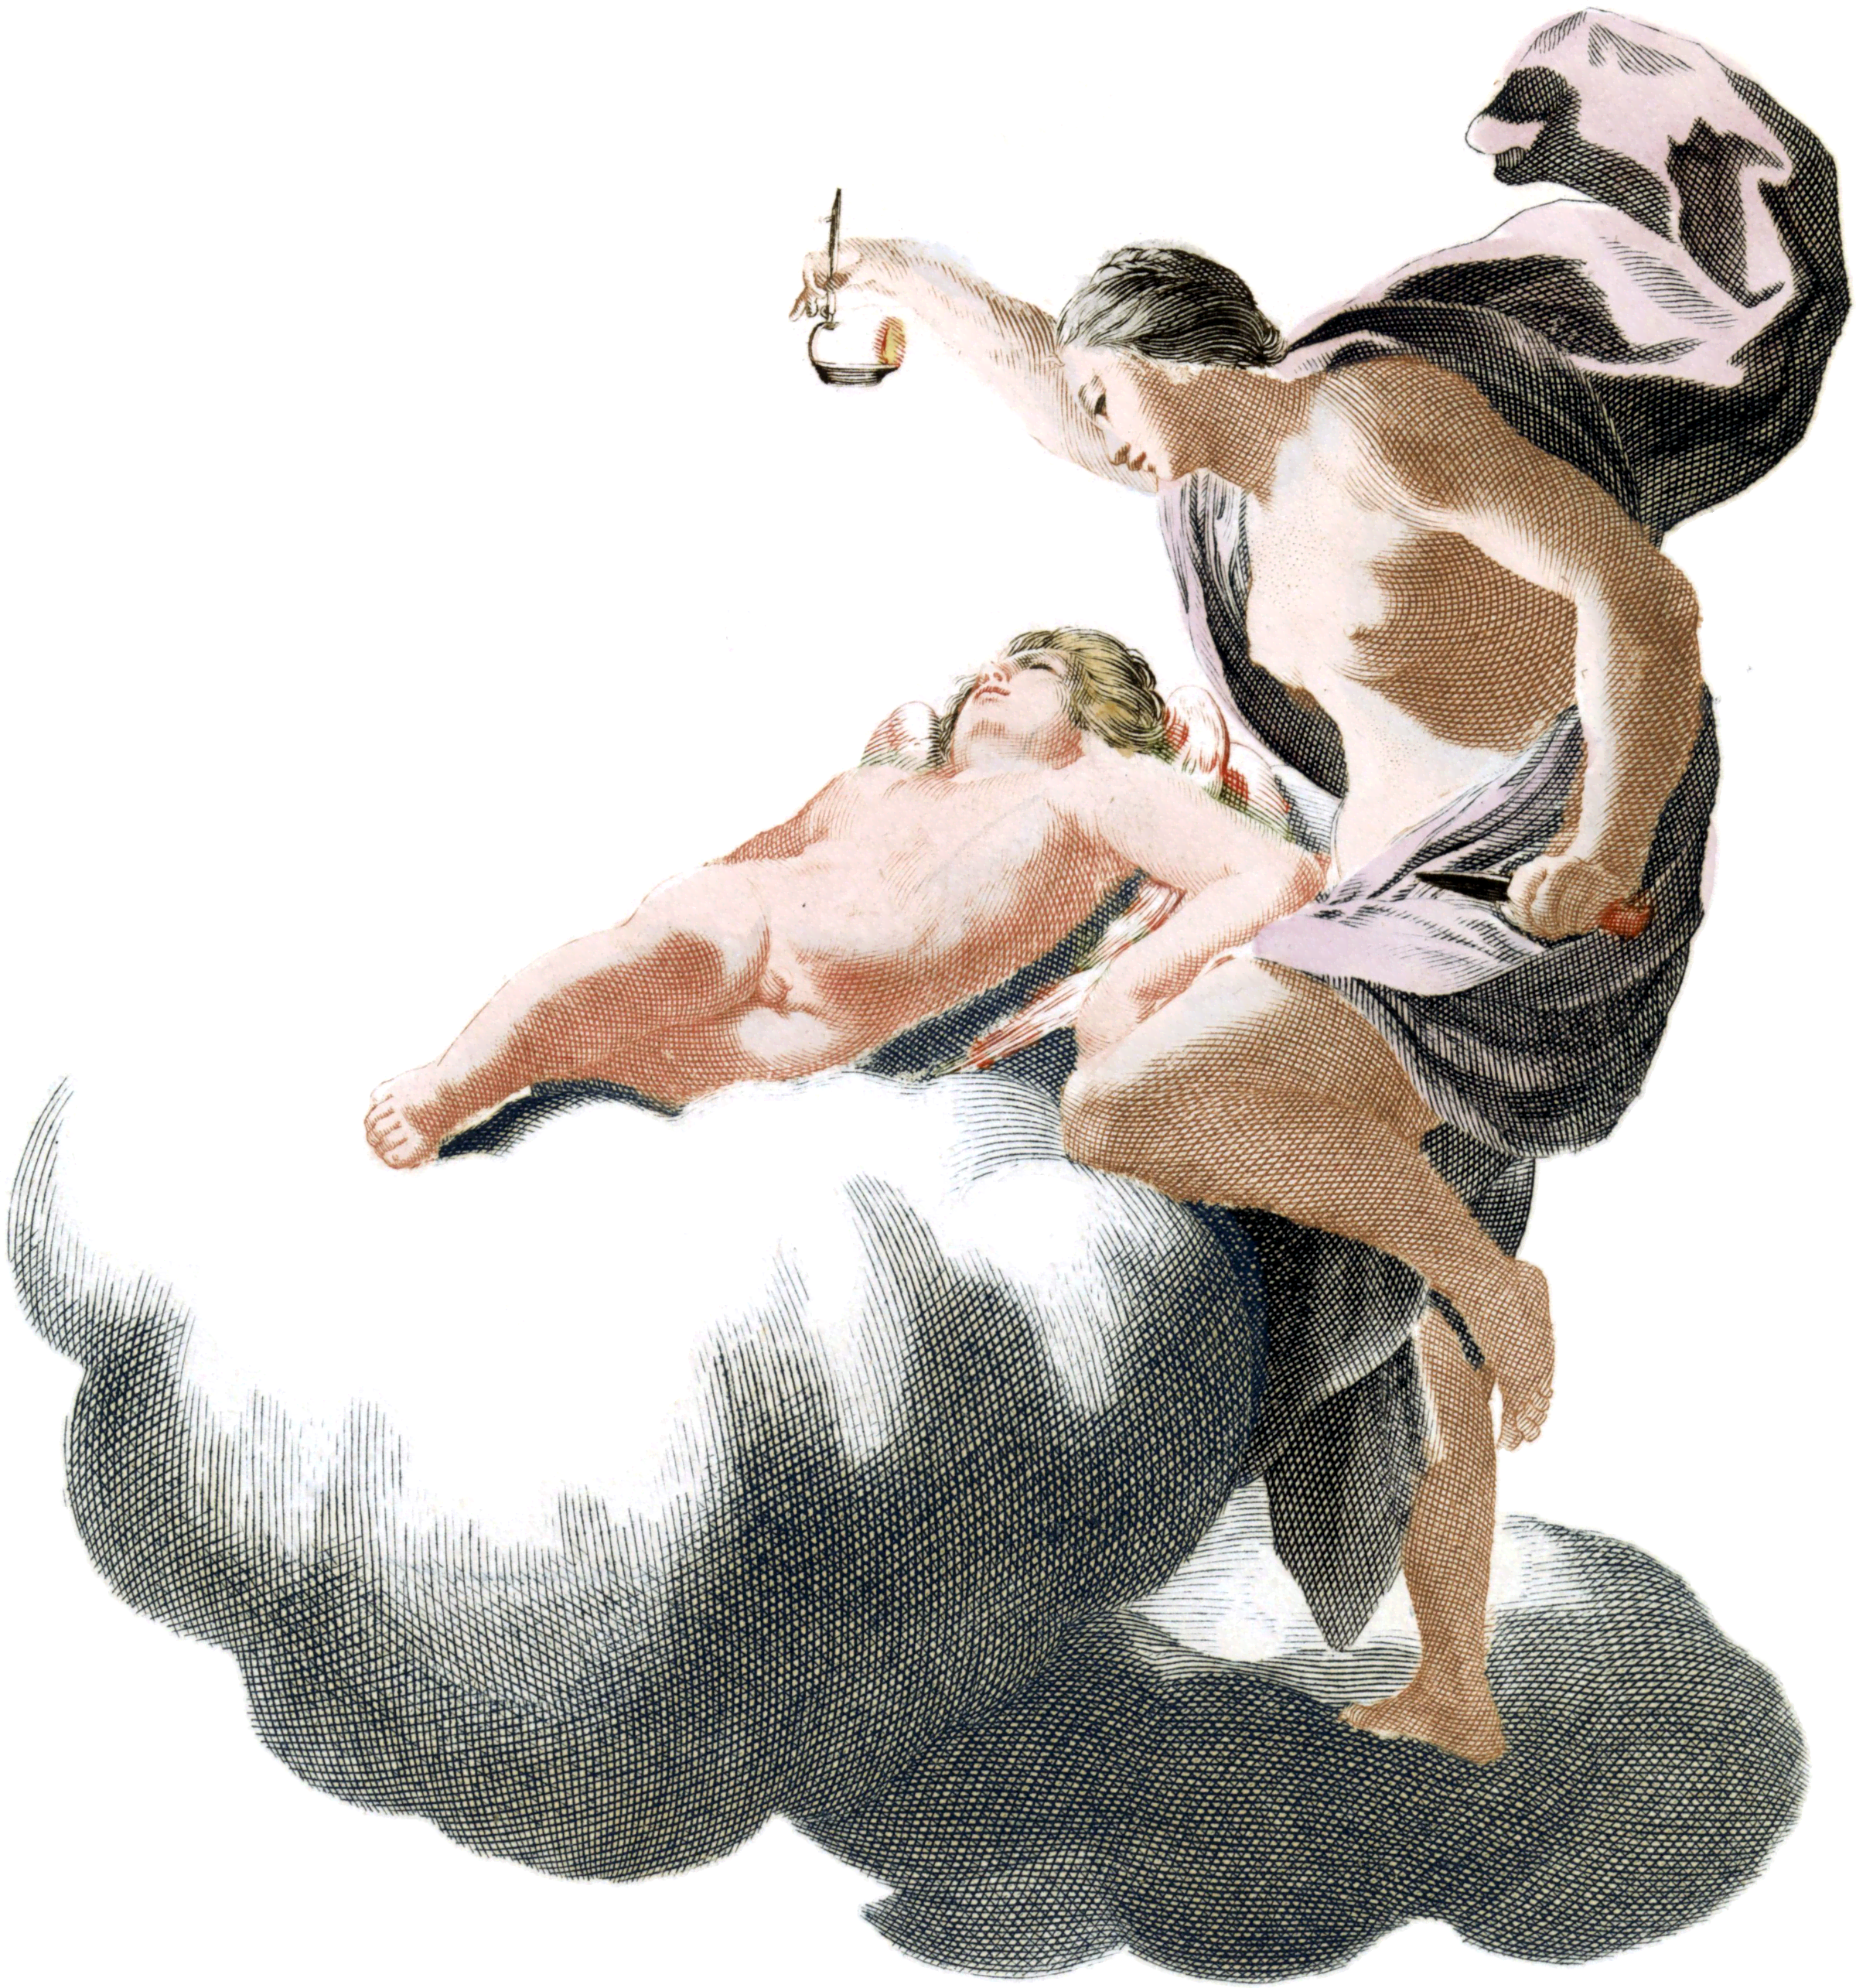
\includegraphics[width=\textwidth,totalheight=\textheight,keepaspectratio]{apuleius_cupid_and_psyche.png}
\end{figure}

But Psyche, terrified at the amazingly beautiful countenance of the God,
impotent of mind, sinking through deadly paleness, and trembling, fell on her
knees, and could not tell where so properly to hide the steel, as in her own
bosom, which, indeed, she would have done, had not the razor, afraid of a crime
so prodigious, fled just then out of her rash hand. And now, as she kneels
weary on the ground, by often beholding the beauty of his divine countenance,
she finds herself refreshed. She sees the genial locks of his golden head,
largely anointed with ambrosia; the ringlets gracefully entangled, wandering
over his milky neck and purple cheeks, some pendulous before, and some behind,
by whose excessive radiance the very light of the lamp shone with a wavering
splendour. On the shoulders of the volatile God, wings of a shining whiteness
were seen; and though they were not in motion, yet the outward tender and
delicate down, tremulously rebounding, was unquietly wanton. The rest of his
body was smooth and elegant, and such as Venus did not repent of bringing
forth. At the foot of the bed lay his bow, his quiver, and his arrows, the
propitious weapons of the mighty God.

These while Psyche with an insatiable mind handles, and explores with eager
curiosity, and admires her husband's arms, she draws out of the quiver one of
the arrows, and with the tip of her finger touching the point to try its
sharpness, by the bold pressure of her trembling hand she pierced the flesh so
deep, that some small drops of rosy blood spread themselves with dewy
sprinkling on her skin; and thus ignorant Psyche voluntarily fell in love with
\textsc{love}. Then, burning more and more with the desire of Cupid, gazing on
his face with insatiable eyes, and multiplying pendulant kisses, her only fear
was, lest he should wake too soon.

But while, astonished through such a mighty good, her wounded mind fluctuates,
the lamp, whether through vile perfidy, or noxious envy, or whether it longed
to touch, and as it were, kiss such a beautiful body, threw out a drop of
boiling oil from the summit of its light on the right shoulder of the God.
Strange, O bold and rash lamp, that thou shouldst burn the very God of all
fire, though some lover first invented thee, that he might for a longer time
enjoy by night the object of his desire. The God, thus burnt, leaped from the
bed, and seeing the evidence of forfeited fidelity, silently flew away from
the eyes and hands of his most unhappy wife. But Psyche immediately, with both
her hands, caught hold of his right leg as he was mounting, being the miserable
appendix of his sublime flight through the cloudy regions, till at length,
through weariness, she fell to the ground.

Her lover God, however, not yet deserting her, as she lay on the ground, flew
to a neighbouring cypress tree, and being severely agitated, thus spoke to her
from its lofty top: ``Most simple Psyche, I, unmindful of the commands of my
mother Venus, who ordered me to cause you to be enamoured of some mean and
miserable son of the vulgar, chose rather to fly to you as a lover myself. I
know that I have acted in this respect lightly, and I, who am so excellent an
archer, have wounded myself with my own arrow, and have made you my wife, that
I might, it seems, be considered by you as a beast, and that you might cut off
my head, which bears those very eyes by which you are beloved. This was the
danger of which I so often warned you to beware; this was the mischief I so
benevolently admonished you to consider. But those egregious counsellors of
yours shall speedily suffer from me the punishment of such pernicious advice;
while you I shall only punish by my flight.'' Thus spake Cupid, and with the
conclusion of his speech sprang with his pinions on high.

But Psyche lay prostrate on the ground, gazing on her soaring husband as long
as he remained in sight, and afflicting herself with lamentations in the
extreme. When, however, by the rowing of his wings, distance had rendered him
invisible, she threw herself from the bank of the next river headlong into its
stream. But the gentle river, in honour of the God, who used to burn the waters
themselves, and fearing for himself, immediately, on the back of an innoxious
wave, delivered her safe to the flowery bank.

It happened at that time, that the rural God Pan sat on the margin of the
river, embracing the Goddess Canna,\footnote{This alludes to the well-known
fable of Syrinx and Pan.} and teaching her to sing in all manner of gentle
strains. Near them a wanton herd of kids browsed on the grassy bank. The
shagged God, who was not ignorant of the misfortune of Psyche, called her
gently to him, and thus allured her in soothing language: ``Most elegant girl,
I am indeed a rural person, and a shepherd; but through the benefit of an
extended old age I have acquired abundance of experience; and if I rightly
conjecture, since prudent men boast the power of divination, from your
stumbling and often reeling gait, from the extreme paleness of your
countenance, from your perpetual sighing and sorrowful eyes, you labour under
an excess of love. Listen, therefore, to me; attempt no more to drown yourself,
or to put an end to your existence by calling any other kind of death to your
assistance; but cease to grieve, lay aside your sorrow, and rather by prayers
worship Cupid, the greatest of the Gods, and strive to please him by bland
obsequiousness, as he is a delicate and luxurious youth.''

The pastoral God having thus spoken, Psyche made no reply, but adoring the
salutary divinity, departed from the place. But before she had travelled far,
with painful steps pursuing an unknown path, she drew near to a city in which
the husband of one of her sisters was king. This, as soon as she understood,
she desired that her arrival might be announced to her sister. Psyche was
accordingly introduced to her, and when the embraces of mutual salutation were
over, to her sister inquiring the cause of her visit, she thus began: ``You
doubtless remember the advice you gave me, I mean, that I should destroy with a
razor the beast that lay with me under the name of a husband, before, through
voracious gluttony, he destroyed me: but as soon as, by the assistance of the
conscious light, I beheld his countenance, I saw a spectacle perfectly
wonderful and divine, the very son himself of the Goddess Venus, Cupid himself
I say, sunk in gentle sleep. And while struck with astonishment at the sight of
such a mighty good, and disturbed through too great an abundance of pleasure, I
laboured under the want of enjoyment, by a most dire misfortune, the boiling
oil bubbled to the summit of the lamp, and leaped on the shoulder of the God.
Being immediately awakened by the pain, when he beheld me armed with weapon and
light, `From whence,' said he, `proceeds this dire wickedness of thine?
Immediately quit my bed, and depart from my sight. I will now immediately join
myself in marriage to your sister,' (mentioning you expressly by name,) and
then he ordered Zephyr to blow me beyond the boundaries of his habitation.''

Psyche had scarcely ended her narration, when the sister, agitated by the
incentives of lust and baneful envy, having deceived her husband by a
preconcerted fiction respecting the death of her parents, immediately set sail
for the rock on which Psyche had been exposed; and though another wind then
blowed, yet, elated with blind hope, she exclaimed, ``Receive me, Cupid, a wife
worthy of thy embraces; and thou, Zephyr, receive thy mistress.'' Then leaping
up as high as she was able, she fell headlong from the mountain, unable even
when dead to arrive at the palace of Cupid. For her limbs were torn in pieces
by the rocks as she fell, and her bowels became, as they deserved to be, food
for birds and beasts of prey. Nor was the vengeance which remained to be
inflicted slow in its approaches: for Psyche with wandering steps arrived at
another city, where her other sister reigned, who, deceived, and sinning in the
same manner, hastened to the rock, and died just in the same way her sister had
done before.

In the meantime, while Psyche wandered over various realms, anxiously searching
after Cupid, he, through the pain of the wound from the lamp, lay groaning in
the bedchamber of his mother. Then that extremely white bird, the sea-gull, who
swims with his wings on the waves of the sea, hastily merged himself in the
profound bosom of the ocean. There, placing himself near Venus, as she was
bathing and swimming, he informed her that her son was severely burnt, that he
was groaning with the pain of the wound, and that his cure was doubtful. That,
besides this, the whole family of Venus was every where reviled; in the first
place, Cupid, because he had retired to a mountain, in order to have illicit
connextion with a girl; and, in the next place, said he, yourself, by thus
withdrawing to swim in the sea. Hence it is said, continued the bird, that
there is no longer any pleasure, elegance, and festivity to be found, but that
every thing is inelegant, rustic, and horrid; that nuptial ties, social
friendships, and love of children, are no more; but that in their place have
succeeded enormous filth, and the bitter loathing of sordid compacts. Thus did
this loquacious and impertinent bird defame the son of Venus, by murmuring
scandal in her ear.

But Venus, being enraged at the information, suddenly exclaimed, in a firm tone
of voice, ``So, then, this hopeful son of mine has got a mistress! Come, tell
me, thou who alone dost serve me with affection, tell me the name of her who
has solicited the ingenuous and naked boy, and whether she is one of the tribes
of Nymphs, or of the number of the Goddesses, or of the choir of the Muses, or
belonging to my train of the Graces?'' The locquacious bird was not silent:
``But, my mistress,'' said he, ``I am not certain, though, if I well remember,
he is said to have been vehemently in love with a girl, whose name is Psyche.''
Then Venus, being indignant, exclaimed, ``Does he then love her who is the
rival of my beauty, and who is emulous of my name? And does he mean to make me,
who first brought him to the knowledge of her, act the part of a bawd?''

Thus complaining, she immediately emerged from the sea, and hastened to her
golden bedchamber, where she found her son sick, as she had been told, and so
vehemently raving through the pain, that she heard him before she reached the
doors. ``This is fine conduct, indeed!'' said she, ``and very agreeable to
\textit{our} dignified birth, and \textit{your} temperance. In the first place,
that you should trample on the precepts of your mistress and mother, and, so
far from tormenting my enemy with sordid love, take her to your licentious and
immature embraces, on purpose that I might suffer the indignity of having my
enemy for my daughter-in-law. Doubtless thou dost presume, thou trifler,
corrupted and unbeloved boy, that I am too old to have another son. Know,
therefore, that I will beget another son, much better than thou art; or rather,
that you may be more sensible of the disgrace, I will adopt one of my little
slaves, and on him will I bestow those wings and flames, that bow, and those
arrows, and all my furniture, which I gave you for purposes very different from
those to which you employ them: for you received no part of this apparatus from
your father's possessions. But thou hast been of a perverse disposition from
thy very childhood, and hence it is that thou hast so often struck thy elders,
and even thy mother herself, even me, thou parricide. Besides, you despise me
as if I were a widow; nor are you afraid of your valiant father-in-law, the
mighty warrior God, whom, to my torment, you have supplied with many a virgin.
I shall take care, however, to make you repent of this frolicsome trick of
yours, and render your nuptials sharp and bitter.

``However, being thus derided, what shall I do? Where shall I betake myself?
How shall I punish that little deceiver? Shall I solicit assistance of my enemy
Sobriety, whom I have so often offended, through the luxury of this fraudulent
boy? Must I have recourse to that rustic and filthy woman? I abhor the very
thought; yet the consolation of revenge is not to be despised. I must therefore
apply to her, and to her alone; for she will most severely chastise this
trifler. She will rifle his quiver, disarm his arrows, unbend his bow,
extinguish his torch, and punish his body with still sharper remedies. Then I
shall believe atonement has been made for the injury I have received, when I
have shaved off those locks, which, with these hands of mine, I have so often
bound with a golden bandage, and cut off those pinions, which I have dyed in
that nectareous fountain, my bosom.''

Having thus given vent to her passion, full of venereal bile, she rushed
impetuously out of doors. But Ceres and Juno immediately attended her, and,
perceiving her angry countenance, asked her why she did so great an injury to
the gracefulness of her sparkling eyes, by such a sullen contraction of her
brows? To whom Venus thus replied: ``You are come very opportunely to be the
executioners of that violence which has taken possession of my ardent breast. I
beg, therefore, that with the utmost care and diligence you will inquire after
the fugitive Psyche; for the infamous report respecting my house, and the
conduct of my unworthy son, cannot be unknown to you.''

Then the two Goddesses, being ignorant of what had happened, thus endeavoured
to mitigate the raging anger of Venus: ``What offence has your son committed,
that you so violently oppose his pleasures, and are impatient to destroy her
whom he loves? What crime, we beseech you, can he be charged with in loving,
without restraint, a beautiful virgin? Can you be ignorant of his sex and
youth? Or have you, indeed, forgot how old he is? What, because he carries his
years elegantly, would you always consider him as a boy? Is it possible, that
you, who are his mother, and besides this a woman of understanding, can be
determined always to pry inquisitively into his sport, blame his luxury and
amours, and reprobate, in your beautiful son, your own arts and delights? But
what God or man will suffer you to disseminate every where among the people
amorous desires, when you restrain the gallantry of your own house, and thus
shut up the public shop of female vices?'' The fear of his darts induced them
to pay this flattery to absent Cupid, in a gracious patronage of his cause. But
Venus, indignant that her injuries were thus ridiculously treated, with haughty
mien and hasty step, passed on to the ocean.

In the meantime, Psyche was driven about from place to place, variously
wandering, and with restless mind inquiring after her husband; her desire of
finding him increasing in proportion to the difficulty of the search. For,
though she had incurred his anger, she hoped she should be able to appease him
by suppliant prayers, if she could not allure him by the tender blandishments
of a wife. Perceiving, therefore, a temple on the summit of a lofty mountain,
``How can I tell,'' said she, ``but this may be the residence of my lord;'' and
immediately she directed her hasty steps thither, incited by hope and desire,
though spent with unceasing toil. And now, having gained the highest ridges of
the mountain, she enters the temple, in which she saw ears of corn, some of
which lay in a heap, some were twisted into garlands, and some were mingled
with ears of barley. Here, likewise, were scythes, and all the instruments of
harvest, but scattered in a confused and careless manner, and thrown, as is
usually the case in the heat of summer, out of the weary hands of the reapers.

Psyche, on seeing this confusion, curiously separated the mingled heaps, and
properly arranged them, when separated, believing that she ought not to neglect
the temples and ceremonies of any divinity, but that she should implore the
benevolent pity of all the Gods. The bountiful Ceres, whose temple this was,
finds her thus anxiously and sedulously employed, and addresses her, at a
distance, as follows: ``Alas! miserable Psyche, Venus, full of rage and
indignation, inquires after thy footsteps with anxious search, dooms thee to
the most severe punishment, and importunately demands revenge, with all the
powers of her divinity. Canst thou therefore now busy thyself about my affairs,
or think of any thing else but thy own safety?''

Then Psyche, throwing herself at the feet of the Goddess, watering them with
abundant weeping, and sweeping the ground with her dishevelled locks, entreated
pardon of her divinity with numerous prayers. ``I beseech thee,'' says she,
``by thy fruit-bering right hand, by the joyful ceremonies of harvest, by the
occult sacred concerns of the cist{\ae}, by the winged car of thy ministrant
dragons, the furrows of the Sicilian soil, the rapacious chariot, and the
detaining earth, by the dark descending ceremonies attending the marriage of
Proserpine, and the ascending rites which accompanies the luminous discovery of
thy daughter, and by other arcana which Eleusis, the Attic sanctuary, conceals
in profound silence,\footnote{See my Dissertation on the Eleusinian and Bacchic
Mysteries.} support the soul of Psyche thy suppliant! Suffer me to conceal
myself in that heap of corn, for a few days, till the raging anger of so great
a Goddess is mitigated by time; or at least permit me to stay here till my
bodily powers, weakened by long-continued labour, become invigorated by an
interval of rest.''

To this prayer Ceres thus replies: ``I am moved by your weeping supplications,
and desire to assist you; but I cannot with propriety incur the displeasure of
a kindred Goddess, to whom I am united by an ancient league of friendship.
Depart, therefore, from this temple immediately, and take in good part my not
detaining you and making you a prisoner.''

Psyche, being thus repulsed, contrary to her hopes, and oppressed with a double
sorrow, retired from the temple, and in a dark grove of the valley, beneath the
mountain, beheld a fane of elegant structure; and, unwilling to omit any way,
though dubious, which might lead to better hope, and determined to implore the
pardon of every God, she suppliantly approached the sacred doors. Here she
perceived splendid gifts, and parts of garments interwoven with golden letters,
fixed to the branches of the trees, and the pillars of the temple; the letters
signifying, that these were votive offerings for benefits received, and
exhibiting the name of the Goddess to whom they were dedicated.

Then Psyche, throwing herself on her knees, and embracing the altar, having
first wiped away her tears, thus prayed: ``O sister and wife of the mighty
Jupiter! whether thou dost possess the ancient temples of Samos, which glories
in the querulous infancy, and in thy nurture; or whether thou dost frequent the
blessed seats of the happy Carthage, which adores thee as a virgin, riding
through the heavens in a lion-yoked car; or dost preside over the illustrious
walls of the Argives, near the banks of Inachus, which celebrates thee now
married to the Thunderer, and Queen of the Gods! O! thou whom all the east
venerates under the name of Zygia, and all the west denominates Lucina! be
thou, Juno, the saviour in this my extreme misfortune, and deliver me, weary
with the toils of such long-continued labours, from the fear of my present
impending danger; for I know that thou are accustomed voluntarily to relieve
the distresses of the pregnant.''

Juno immediately presented herself to Psyche supplicating, in all the august
dignity of her divinity, and said, ``I would most willingly have my
daughter-in-law, Venus, yield to your prayers; but decency will not permit me
to act contrary to the will of Venus, whom I have always loved as my own
daughter. Besides, the law forbids me to receive into my protection any
fugitive servant, without the consent of her mistress.''

But Psyche, now terrified with this second shipwreck of her fortune, and
despairing of being able to recover her volatile husband, having laid aside all
hope of safety, thus consulted with her own thoughts. ``What other relief for
my sorrows can now be either attempted or procured since even Goddesses cannot,
though willing, afford me assistance? To what place shall I again direct my
wandering steps, when entangled in such inextricable nets? Concealed in what
habitations or darkness, can I escape the inevitable eyes of the mighty Venus?
Assume, therefore, a masculine mind, my soul, bravely renounce all thy vain
little hopes, voluntarily surrender thyself into the hands of thy mistress, and
try, though late, to mitigate her rage by the modesty of thy behaviour.
Besides, thou mayest perhaps find him in the house of his mother, whom thou
hast so long sought for in vain.'' Being thus prepared to enter on her dubious
duty, or rather certain destruction, she considered with herself how she should
begin her supplications to Venus.

Venus, however, refusing to employ earthly remedies in her inquiries after
Pscyhe, returned to heaven. She orders the chariot to be made ready, which
Vulcan, having fabricated with subtle skill, arched like the horned moon, and
precious with a waste of gold, had presented her before the consummation of her
marriage. Four white doves, out of many that nestled about the bedchamber of
their mistress, joyfully turning about their painted necks, assume the yoke,
decorated with gems, and, having taken up their mistress, gladly fly with her
to heaven. The chariot of the Goddess was attended by a flock of sparrows,
wantoning with loud chirpings, and by other birds who sing sweetly; all of them
announcing the approach of Venus in the most mellifluous notes.

The clouds give way, the heavens unfold themselves to their daughter, and the
lofty {\ae}ther receives the Goddess with joy; nor does the singing family of
Venus fear opposing eagles, or rapacious hawks. Then immediately she directed
her steps to the royal palace of Jupiter, and proudly demanded the necessary
assistance of the vocal God Mercury; nor did the azure brow of Jupiter refuse
assent. Then Venus, accompanied by Mercury, joyfully descended from heaven,
and, in her flight, thus anxiously addressed him: ``My Arcadian brother, you
well know that your sister, Venus, never did any thing without the presence of
Mercury, nor are you ignorant how long I have sought in vain for my lurking
female slave. Hence nothing remains to be done, but for you to proclaim her in
a public manner, and propose a reward to him that shall find her. Take care,
therefore, that my commands are speedily executed, and clearly describe the
marks by which she may be known, that no one may plead ignorance for the crime
of unlawfully concealing her.'' At the same time, she gave him a small volume,
in which the name of Psyche was written, and every other particular respecting
her, after which she immediately returned home. Nor was Mercury negligent in
the performance of her commands; for, running every where, through all nations,
he cried her in the following words: \textsc{``If any one can seize in her
flight, or discover where a fugitive king's daughter, a servant of Venus, and
of the name of Psyche, lies concealed, let him or her repair to Mercury, the
crier, at the temple of Venus Murtia,\footnote{So called from the myrtle tree,
which is sacred to Venus.} and receive, as a reward of the discovery, seven
sweet kisses from Venus herself, and one exquisitely delicious touch of her
charming tongue.''}

Mercury having thus executed the proclamation of Venus, the desire of such a
mighty reward excited ardent endeavours in all mortals to obtain it, and this
circumstance took away from Psyche all thoughts of further delay. And now, as
she approached the gates of her mistress, she was met by one of the servants of
Venus, named Custom, who immediately exclaimed, as loud as she was able, ``At
length, then, most wicked slave, do you begin to know that you have a mistress?
And do you likewise pretend to be ignorant of the great fatigue we have endured
in endeavouring to find you out? But it is well that you have fallen into my
hands; for now you have entered the very gates of hell, to receive, without
delay, the punishment of such obstinate contumacy.''

After she had thus reviled Psyche, she audaciously twisted her hands in her
hair, and dragged her along without resistance. But Venus, as soon as she
beheld her thus brought into her presence, burst into a loud laugh, such as
agitates those who are transported with vehement rage; and, shaking her head,
``At length,'' says she, ``have you thought proper to come and pay your
respects to your mother-in-law? Or did you rather come to see your sick
husband, who is yet dangerously ill through the wound which you gave him? But
take courage, for your reception will be such as a good mother-in-law ought to
give. Where then,'' said she, ``are my servants Solicitude and Sorrow?'' These,
immediately attending, in obedience to the commands of their mistress, scourged
and inflicted other torments on the miserable Psyche, and afterwards brought
her again into the presence of Venus.

Then Venus, again laughing: ``Behold,'' said she, ``her swelling belly moves my
compassion, since it is through this that she is to make me a happy
grandmother. Happy, indeed, am I, who, in the very flower of my age, shall be
called a grandmother! And the son of a vile slave shall be dignified with the
appellation of the grandson of Venus! Though, indeed, I foolishly call him my
grandson; for marriages unequal, and, besides this, made in a village, without
any witnesses, and without the father's consent, can never be deemed
legitimate; so that thy offspring must be a bastard, even if I should suffer
thee to bring him into the light.''

Having thus said, she flew upon her, rent her garments in many places, tore her
hair, beat her on the head, and severely chastised her in various ways. Then,
taking wheat, barley, millet, poppy-seed, vetches, lentils, and beans, and,
mixing them into one globular heap, she thus spoke to her: ``You seem to me a
servant so deformed, as to be incapable of deserving your lover by any other
means than the diligent performance of menial employments. I will, therefore,
myself make trial of your abilities as a housewife. Take and separate this mass
of seeds, and having properly disposed the several grains apart from each
other, give me a proof of your expedition, by finishing the task before
evening.'' Thus spoke Venus, and immediately after departed to a wedding
supper.

But Psyche, astonished at the prodigious command, sat silent and stupid,
without moving a hand to the disordered and inextricable mass. Then a little
ant, a native of the fields, vehemently commiserating such prodigious
difficulty and labour, and execrating the step-mother's cruelty towards the
wife of the mighty God Cupid, rapidly summoned together the populous tribe of
neighboring ants, and thus addressed them: ``Take pity, ye active nurslings of
the all-parent earth! Take pity, and with prompt celerity assist the wife of
Love, a beautiful young woman, who is now in a dangerous situation.''

Immediately the six-footed people rushed forth to her assistance in undulating
tribes, and with the utmost diligence separated the whole heap, grain by grain,
and, having properly sorted the confusedly mingled species, rapidly vanished
from her sight.

But Venus, on the commencement of night, returns from the nuptial banquet,
moist with wine, fragrant with rich ointments, and having her body elegantly
bound with shining roses. And as soon as she saw the diligence which had been
exerted on the wonderful labour, ``Most vile creature,'' said she, ``this is
not the work of your hands, but of his whom, to your own and his misfortune,
you have pleased;'' and throwing her a piece of household bread, she retired to
rest.

In the meantime, Cupid was very closely confined to his bedchamber, in the
interior part of the house, partly lest he should injure his wound by petulant
luxury, and partly lest he should associate with his beloved. Thus the lovers,
being separated from each other under one roof, passed away, exhausted with
grief, the cruel night. But as soon as Aurora had ushered in the morning, Venus
having called Psyche, thus addressed her: ``Do you perceive yonder grove which
stretches itself to a considerable distance along the margin of a river, whose
deepest whirlpools look down upon a neighbouring fountain? There shining sheep
of a golden colour wander about, feeding without a shepherd. I think it fit
that you should bring me immediately a flock of that precious wool, whatever
may be the difficulty of procuring it.''

Psyche willingly rose, not with any intention of executing this command, but to
procure rest from her misfortunes, by hurling herself headlong from the rock
into the river. But when she came to the brink, a reed, the sweet nurse of
music,\footnote{So called because the pipe of Pan was formed of reeds joined
together.} being divinely inspired, thus prophetically spoke in soft and
harmonious murmurs: ``Psyche! exercised in mighty sorrows, neither pollute my
sacred waters by thy most miserable death, nor yet venture to approach the
formidable sheep on the opposite bank, while, borrowing heat from the burning
radiance of the sun, they are transported with savage rage, and are the
destruction of mortals, either by their sharp horns, stony foreheads, or
venemous bites. But when the meridian sun has driven the cattle to the shade,
and the serene spirit of the flood lulled them to rest, then you may hide
yourself under yonder lofty plane tree, which drinks of the same river with
myself, and as soon as the sheep have mitigated their fury, on shaking the
leaves of a neighbouring grove, you will find the wooly gold every where
sticking to the roots of the trees.'' Thus the simple and humane reed taught
the wretched Psyche how to accomplish this dangerous enterprise with safety.

Psyche, therefore, observing all the directions, found her obedience was not in
vain, but returned to Venus with her bosom full of the delicate golden fleece.
Yet she was not able to procure the approbation of her mistress by this her
second perilous labour. But Venus, smiling bitterly with severe eyebrows, thus
addressed her: ``I am not ignorant that you are not the performer of this task
also; but I will now try whether you are endued with a courageous mind and
singular prudence. Do you see the summit of yonder lofty mountain, from which
the dusky waters of a black fountain fall, and which, confined in the channel
of the neighbouring valley, irrigate the Stygian marshes, and supply the hoarse
streams of Cocytus? Bring me immediately in this little urn, liquid dew drawn
from the most inmost influx of the lofty fountain.'' Thus speaking, she gave
her a vessel of polished crystal, and at the same time threatened her more
severely than before.

But Psyche, with the utmost celerity, ascended to the very summit of the
mountain, presuming that there at least she should find the period of her most
miserable life. However, when she arrived at the confines of the vertex, she
saw the deadly difficulty of the vast undertaking. For a rock enormously
lofty, and inaccessibly rugged, vomited from its middle the horrid waters of
the fountain, which, immediately falling headlong in winding streams, rushed
suddenly through a narrow channel into the neighbouring valley. On the right
and left hand they creep through hollow rocks, over which fierce dragons
stretch out their long necks, and with unwinking vigilance keep a perpetual
watch. And now the vocal waters shook themselves, and exclaimed as they rolled
along, ``Depart; what do you attempt? Look and see what you do; take care, fly,
or you will perish.''

Psyche, therefore, petrified through the impossibility of accomplishing the
task, though she was present in body, was absent in mind, and being perfectly
buried under the huge bulk of the inextricable danger, was even deprived of the
benefit of tears, the last solace of the wretched. But the sorrow of the
innocent soul is not concealed from the penetrating eyes of Providence. For the
rapacious eagle, that royal bird of Jupiter, on a sudden flew to her with
expanded wings, calling to mind his ancient obligations to Cupid, for enabling
him to elevate to heaven the Phrygian cup-bearer [Ganymedes] to Jupiter; and
reverencing the divinity of Cupid, in the labours of his wife, deserted the
lofty paths of Jupiter, and bringing with him seasonable assistance, thus
addressed her: ``Can you, in other respects of an undesigning disposition, and
unexperienced in attempts of this kind, ever hope to steal one drop of this
most holy and no less terrible fountain? Have you not heard, at least, that
these Stygian waters are formidable even to Jupiter himself, and that as you
swear by the divinity of the Gods, so they are accustomed to swear by the
majesty of the Styx?\footnote{Styx, considered according to its first
subsistence, appears to me to be that cause by which divine natures retain an
immutable sameness of essence. The immutability, therefore, of divine energy,
is signified by the Gods swearing by the Styx.} But give me that little urn.''
Immediately, therefore, taking it in haste and poising it on his moving wings,
he sailed between the cheeks of raging teeth, and the three-forked vibrating
tongues of the dragons, and steering his course to the right and to the left,
drew off the reluctant waters, which previously admonished him that he might
depart in safety, because he pretended that Venus herself wanted some of the
water, and had ordered him to procure it. And on this account, his access to
the fountain was facilitated.

Psyche, therefore, joyfully receiving the full urn, returned with the utmost
celerity to Venus. Yet she was not able, even by the accomplishment of this
dangerous enterprise, to appease the anger of the raging Goddess. For,
threatening her with still more severe endurance, she thus addressed her, a
smile, the harbinger of ruin, accompanying her words: ``You appear to me to be
a profound and malevolent magician, or you never could with so much dexterity
have performed my commands: but there is one task more, my dear, which you
ought to perform. Take this box,'' (she immediately gave it to her), ``and
direct your course to the infernal regions and the deadly palace of Pluto. Then
presenting the box to Proserpine, say, Venus requests you to send her a small
portion of your beauty, at least as much as may be sufficient for one short
day; for she has consumed all the beauty she possessed, through the attention
which she pays to her diseased son. But return with the utmost expedition; for
it is necessary that I should adorn myself with this beauty of Proserpine, as I
must go to the theatre of the Gods.''

Psyche was now truly sensible, that she was arrived at the extremity of her
evil fortune; and clearly perceived that, all further pretences being laid
aside, she was impelled to immediate destruction, since she was forced to
direct her steps to Tartarus and the shades below. Hence, without any farther
delay, she ascended a lofty tower, that she might from thence hurl herself
headlong: for she considered that she should thus descend by a straight road,
and in a beautiful manner, to the infernal regions. But she was no sooner
arrived there, than the tower suddenly addressed her in the following words:

``Why, O miserable creature, dost thou seek to destroy thyself by falling
headlong from hence? And why dost thou rashly sink under this thy last danger
and endurance? For as soon as thy breath shall thus be separated from thy body,
thou wilt indeed descend to profound Tartarus, but canst not by any means
return from thence. Listen, therefore, to me. Laced{\ae}mon, a noble city of
Achaia, is not far from hence. Near this city, concealed in devious places,
seek Tenarus; for there you will find the cavity through which Pluto breathes,
and the impassable road presents itself to the view through the yawning gates.
As soon as you have passed the threshold of this cavity, you proceed in a
direct path to the palace of Pluto. You ought not, however, to pass through
those shades with empty hands, but should take a sop of barley bread, soaked in
hydromel, in both your hands, and in your mouth two pieces of money. And now,
when you have accomplished a good part of your deadly journey, you will meet a
lame ass laden with wood, with a driver as lame as himself, who will ask you to
reach him certain cords to fasten the burden which has fallen from the ass; but
be careful that you pass by him in silence. Then, without any delay, proceed
till you arrive at the dead river, in which Charon, immediately demanding his
fee, in his patched boat ferries over the passengers to the farthest shore.

``Avarice, therefore, lives among the dead. Nor does Charon himself, nor the
father Pluto, though so great a God, do any thing gratuitously. The poor man,
dying, ought to prepare his viaticum; and no one suffers him to expire without
having money at hand. To this squalid old man give one of the pieces of money
which you carry with you; yet in such a manner, that he may take it with his
own hand from your mouth. While you are passing over the sluggish river, a
certain dead old man, floating on its surface, and raising his putrid hand,
will entreat you to take him into the boat. However, be careful that you are
not influenced by an unlawful piety. Having passed over the river, and
proceeded to a little distance from thence, certain old women, weaving a web,
will request you to lend them a helping hand; but it is not lawful for you to
touch the web. For all these, and many other particulars, are snares prepared
for you by Venus, that you may drop one of the sops out of your hands. But do
not suppose that this would be a trifling loss; since the want of only one of
these sops, would prevent your return to light. For a huge dog, with three
necks, and heads sufficiently large, fierce, and formidable, barking with his
thundering jaws, terrifies in vain the dead, whom he cannot injure; and always
watching before the threshold and black palace of Proserpine, guards the empty
house of Pluto. Having appeased this dog with one of your sops, you may easily
pass by him, and then you will immediately enter into the presence of
Proserpine herself, who will receive you in a very courteous and benignant
manner, desire you to repose yourself on a soft seat, and persuade you to
partake of a sumptuous banquet. But seat yourself on the ground, and having
asked for a piece of common bread, eat it. Then telling your message, and
receiving what you came for, bribe the cruelty of the dog by the remaining sop.
Afterwards, having given to the avaricious ferryman the piece of money which
you have reserved, and passed his river, you will return to the choir of the
celestial stars. But, above all things, I think you should particularly be
cautious not to open or even look on the box which you carry, or explore that
concealed treasury of divine beauty.'' In this manner the propitious tower
delivered its prophetic admonitions.

Psyche, therefore, without delay, proceeded to Tenarus, and taking in a proper
manner her pieces of money and her sops, ran down the infernal avenue. Here,
having passed by the lame ass in silence, given the ferryman his fee, neglected
the entreaties of the floating corpse, despised the fraudulent prayers of the
spinsters, and lulled the rage of the horrid dog with a sop, she penetrated the
palace of Proserpine. Nor did she accept the delicate seat, or delicious
banquet; but humbly sat at the feet of Proserpine, and being contented with a
piece of common bread, delivered her embassy from Venus. Immediately after
this, she received the box secretly filled and shut; and having barred the
barking of the dog by the fraud of the remaining sop, and given the ferryman
the other piece of money, she returned from the infernal regions much more
vigorous than before. Then again enjoying and adoring the fair light of day,
though she was in haste to finish her errand, she was seized with a rash
curiosity: ``Behold,'' said she, ``what a foolish bearer am I of divine beauty,
who do not even take the least portion of it, that I may by this means appear
pleasing in the eyes of my beautiful lover.'' As she ended this soliloquy, she
opened the box; but it contained no beauty, nor indeed any thing but an
infernal and truly Stygian sleep, which being freed from its confinement,
immediately invades her, oppresses all her members with a cloud of profound
sleep, and detains her, fallen down in the very place where she opened the box;
so that she lay motionless, and nothing else than a sleeping corpse.

But Cupid, being now recovered of his wound, and not enduring the long absence
of his Psyche, glided through the narrow window of the bedchamber in which he
was confined, and having his wings invigorated by repose, flew far more swiftly
than before; and dispelling the sleep from the prying fair, and again
concealing it in its ancient seat, the box, roused Psyche with an innoxious
touch of one of his arrows. ``And behold,'' said he, ``miserable creature, thou
wouldst again have perished by a similar curiosity. Now, however, strenuously
perform the task imposed on thee by my mother, and I myself with take care of
the rest.'' Having thus spoke, the lover raised himself on high with the rowing
of his wings, and Psyche immediately carried the present of Proserpine to
Venus.

In the meantime, Cupid, wasting away through excess of love, and dreading the
sudden severity of his mother, returns to his armoury, and having with rapid
wings penetrated the summit of heaven, supplicates the mighty Jupiter, and
defends his cause. Then Jupiter, stroking the little cheeks of Cupid, and
kissing his hand, thus addressed him: ``Though you, my son, endued with the
authority of a master, never pay me the reverence which has been decreed me by
the synod of the Gods, but perpetually wound this breast of mine, by which the
laws of the elements and the revolutions of the stars are governed, and
frequently defile it with earthly intrigues, contrary to the laws, the Julian
edict,\footnote{Alluding to the law against adultery, instituted by Augustus
C{\ae}sar.} and public discipline, injuring my reputation and fame by base
adulteries, and sordidly changing my serene countenance into serpents, fire,
wild beasts, birds, and cattle; yet remembering my own moderation, and that you
have been nursed in these hands of mine, I will accomplish all that you desire;
and at the same time you must be sensible that you ought to guard against your
rivals, and to recompense me for this service, by presenting me with any girl
of transcendent beauty that may now happen to be upon the earth.''

Having thus spoke, he ordered Mercury immediately to summon all the Gods to
attend; and at the same time to proclaim, that, if any one of the celestials
was absent, he should be fined ten thousand pieces of money. Through fear of
this, therefore, the celestial theatre being immediately filled, lofty Jupiter,
sitting on his sublime throne, thus addressed the assembly of Gods: ``Ye
conscript Gods, whose names are registered in the white roll of the Muses, you
are all well acquainted with that youth whom I have reared with my own hands,
and the fiery impetus of whose first years I thought would have been restrained
by some bridle or other. It is sufficient that he is every day defamed in
conversation, for the adulteries and all manner of corruption of which he is
the cause. Every occasion of this is to be taken away, and his puerile luxury
ought to be bound in nuptial fetters. He has made choice of a girl, and
deprived her of her virginity. Let him, therefore, hold her, let him possess
her, and embracing Psyche, always enjoy the object of his love.'' Then turning
his face to Venus, ``Nor do you, my daughter,'' said he, ``be sorrowful on this
occasion, nor fearful that your pedigree and rank will be disgraced by a mortal
marriage; for I will now cause the nuptials not to be unequal, but legitimate,
and agreeable to the civil law.'' Immediately after this, he ordered Mercury to
bring Psyche to heaven; and as soon as she was arrived, extending to her a cup
of ambrosia, ``Take this,'' said he, ``Psyche, and be immortal; nor shall Cupid
ever depart from thy embrace, but these nuptials of yours shall be perpetual.''

Then, without delay, the wedding supper was served in great abundance. The
husband, reclining at the upper end of the table, embraced Psyche in his bosom;
and in this manner, Jupiter was seated with Juno, and after them, the other
Gods and Goddesses in their proper order. Then Jupiter was presented with a
bowl of nectar, which is the wine of the Gods, by that rustic youth
[Ganymedes], his cup-bearer; but Bacchus supplied the rest. Vulcan dressed the
supper; the Hours purpled over every thing with roses, and other fragrant
flowers; the Graces scattered balsam; the Muses sang melodiously; Apollo
accompanied the lyre with his voice; and Venus beautifully danced with steps in
unison with the delightful music. The order, too, of the entertainment was,
that the Muses should sing the chorus, Satyrus play on the flute, and
Paniscus\footnote{One of the satyrs of the wood.} speak to the pipe. Thus
Psyche came lawfully into the hands of Cupid; and, at length, from a mature
pregnancy, a daughter was born to them, who we denominate Pleasure.

\end{document}
